%% abtex2-modelo-relatorio-tecnico.tex, v-1.9.7 laurocesar
%% Copyright 2012-2018 by abnTeX2 group at http://www.abntex.net.br/ 
%%
%% This work may be distributed and/or modified under the
%% conditions of the LaTeX Project Public License, either version 1.3
%% of this license or (at your option) any later version.
%% The latest version of this license is in
%%   http://www.latex-project.org/lppl.txt
%% and version 1.3 or later is part of all distributions of LaTeX
%% version 2005/12/01 or later.
%%
%% This work has the LPPL maintenance status `maintained'.
%% 
%% The Current Maintainer of this work is the abnTeX2 team, led
%% by Lauro César Araujo. Further information are available on 
%% http://www.abntex.net.br/
%%
%% This work consists of the files abntex2-modelo-relatorio-tecnico.tex,
%% abntex2-modelo-include-comandos and abntex2-modelo-references.bib
%%

% ------------------------------------------------------------------------
% ------------------------------------------------------------------------
% abnTeX2: Modelo de Relatório Técnico/Acadêmico em conformidade com 
% ABNT NBR 10719:2015 Informação e documentação - Relatório técnico e/ou
% científico - Apresentação
% ------------------------------------------------------------------------ 
% ------------------------------------------------------------------------

\documentclass[
	% -- opções da classe memoir --
	12pt,				% tamanho da fonte
	openright,			% capítulos começam em pág ímpar (insere página vazia caso preciso)
	twoside,			% para impressão em recto e verso. Oposto a oneside
	a4paper,			% tamanho do papel. 
	% -- opções da classe abntex2 --
	%chapter=TITLE,		% títulos de capítulos convertidos em letras maiúsculas
	%section=TITLE,		% títulos de seções convertidos em letras maiúsculas
	%subsection=TITLE,	% títulos de subseções convertidos em letras maiúsculas
	%subsubsection=TITLE,% títulos de subsubseções convertidos em letras maiúsculas
	% -- opções do pacote babel --
	english,			% idioma adicional para hifenização
	french,				% idioma adicional para hifenização
	spanish,			% idioma adicional para hifenização
	brazil,				% o último idioma é o principal do documento
	]{abntex2}


% ---
% PACOTES
% ---

% ---
% Pacotes fundamentais 
% ---
\usepackage{lmodern}			% Usa a fonte Latin Modern
\usepackage[T1]{fontenc}		% Selecao de codigos de fonte.
\usepackage[utf8]{inputenc}		% Codificacao do documento (conversão automática dos acentos)
\usepackage{indentfirst}		% Indenta o primeiro parágrafo de cada seção.
\usepackage{color}				% Controle das cores
\usepackage{graphicx}			% Inclusão de gráficos
\usepackage{microtype} 			% para melhorias de justificação
% ---

% ---
% Pacotes adicionais, usados no anexo do modelo de folha de identificação
% ---
\usepackage{multicol}
\usepackage{multirow}
% ---
	
% ---
% Pacotes adicionais, usados apenas no âmbito do Modelo Canônico do abnteX2
% ---
\usepackage{lipsum}				% para geração de dummy text
% ---

% ---
% Pacotes de citações
% ---
\usepackage[brazilian,hyperpageref]{backref}	 % Paginas com as citações na bibl
\usepackage[alf]{abntex2cite}	% Citações padrão ABNT

% --- 
% CONFIGURAÇÕES DE PACOTES
% --- 

% ---
% Configurações do pacote backref
% Usado sem a opção hyperpageref de backref
\renewcommand{\backrefpagesname}{Citado na(s) página(s):~}
% Texto padrão antes do número das páginas
\renewcommand{\backref}{}
% Define os textos da citação
\renewcommand*{\backrefalt}[4]{
	\ifcase #1 %
		Nenhuma citação no texto.%
	\or
		Citado na página #2.%
	\else
		Citado #1 vezes nas páginas #2.%
	\fi}%
% ---

% ---
% Informações de dados para CAPA e FOLHA DE ROSTO
% ---
\titulo{Documento de Conceito Operacional (OpsCon) — Programa Sukatech}
\autor{Brenda Andreia Lima Pinheiro \\ Fabio Tiago Vieira Soares Marques \\ Giovanna Waleska Theodoro Barbosa \\
Yatherson Lucas Theodoro Souza}
\local{Goiânia, Goiás \\ Brasil}
\data{Julho, 2025}
\instituicao{%
  Universidade Federal de Goiás
  \par
  Instituto de Informática
  \par
  Bacharelado em Sistemas de Informação}
\tipotrabalho{Relatório técnico}
% O preambulo deve conter o tipo do trabalho, o objetivo, 
% o nome da instituição e a área de concentração 
\preambulo{Este Documento de Conceito Operacional (OpsCon) apresenta conceitos e aspectos fundamentais sobre o Programa Sukatech para membros da comunidade acadêmica, da administração pública, e do terceiro setor sob a perspectiva da grande área de Sistemas de Informação. Ele consolida observações do grupo de residentes técnicos denominado Squad 2 da turma de 2025-1 da Residência Técnica em Sistemas de Informação.}
% ---

% ---
% Configurações de aparência do PDF final

% alterando o aspecto da cor azul
\definecolor{blue}{RGB}{41,5,195}

% informações do PDF
\makeatletter
\hypersetup{
     	%pagebackref=true,
		pdftitle={\@title}, 
		pdfauthor={\@author},
    	pdfsubject={\imprimirpreambulo},
	    pdfcreator={LaTeX with abnTeX2},
		pdfkeywords={abnt}{latex}{abntex}{abntex2}{relatório técnico}, 
		colorlinks=true,       		% false: boxed links; true: colored links
    	linkcolor=blue,          	% color of internal links
    	citecolor=blue,        		% color of links to bibliography
    	filecolor=magenta,      		% color of file links
		urlcolor=blue,
		bookmarksdepth=4
}
\makeatother
% --- 

% --- 
% Espaçamentos entre linhas e parágrafos 
% --- 

% O tamanho do parágrafo é dado por:
\setlength{\parindent}{1.3cm}

% Controle do espaçamento entre um parágrafo e outro:
\setlength{\parskip}{0.2cm}  % tente também \onelineskip

% ---
% compila o indice
% ---
\makeindex
% ---

% ----
% Início do documento
% ----
\begin{document}

% Seleciona o idioma do documento (conforme pacotes do babel)
%\selectlanguage{english}
\selectlanguage{brazil}

% Retira espaço extra obsoleto entre as frases.
\frenchspacing 

% ----------------------------------------------------------
% ELEMENTOS PRÉ-TEXTUAIS
% ----------------------------------------------------------
% \pretextual

% ---
% Capa
% ---
\imprimircapa
% ---

% ---
% Folha de rosto
% (o * indica que haverá a ficha bibliográfica)
% ---
\imprimirfolhaderosto*
% ---

% ---
% Anverso da folha de rosto:
% ---

{
\ABNTEXchapterfont

\vspace*{\fill}

Conforme a ABNT NBR 10719:2015, seção 4.2.1.1.1, o anverso da folha de rosto
deve conter:

\begin{alineas}
  \item nome do órgão ou entidade responsável que solicitou ou gerou o
   relatório; 
  \item título do projeto, programa ou plano que o relatório está relacionado;
  \item título do relatório;
  \item subtítulo, se houver, deve ser precedido de dois pontos, evidenciando a
   sua subordinação ao título. O relatório em vários volumes deve ter um título
   geral. Além deste, cada volume pode ter um título específico; 
  \item número do volume, se houver mais de um, deve constar em cada folha de
   rosto a especificação do respectivo volume, em algarismo arábico; 
  \item código de identificação, se houver, recomenda-se que seja formado
   pela sigla da instituição, indicação da categoria do relatório, data,
   indicação do assunto e número sequencial do relatório na série; 
  \item classificação de segurança. Todos os órgãos, privados ou públicos, que
   desenvolvam pesquisa de interesse nacional de conteúdo sigiloso, devem
    informar a classificação adequada, conforme a legislação em vigor; 
  \item nome do autor ou autor-entidade. O título e a qualificação ou a função
   do autor podem ser incluídos, pois servem para indicar sua autoridade no
   assunto. Caso a instituição que solicitou o relatório seja a mesma que o
   gerou, suprime-se o nome da instituição no campo de autoria; 
  \item local (cidade) da instituição responsável e/ou solicitante; NOTA: No
   caso de cidades homônimas, recomenda-se o acréscimo da sigla da unidade da
   federação.
  \item ano de publicação, de acordo com o calendário universal (gregoriano),
  deve ser apresentado em algarismos arábicos.
\end{alineas}

\vspace*{\fill}
}

% ---
% Agradecimentos
% ---
\begin{agradecimentos}
Agredecemos ao professor Juliano Lopes de Oliveira pela sua dedicada e anteciosa orientação durante o período da residência técnica. 


\end{agradecimentos}
% ---

% ---
% RESUMO
% ---

% resumo na língua vernácula (obrigatório)
\setlength{\absparsep}{18pt} % ajusta o espaçamento dos parágrafos do resumo
\begin{resumo}
 Segundo a \citeonline[3.1-3.2]{NBR6028:2003}, o resumo deve ressaltar o
 objetivo, o método, os resultados e as conclusões do documento. A ordem e a extensão
 destes itens dependem do tipo de resumo (informativo ou indicativo) e do
 tratamento que cada item recebe no documento original. O resumo deve ser
 precedido da referência do documento, com exceção do resumo inserido no
 próprio documento. (\ldots) As palavras-chave devem figurar logo abaixo do
 resumo, antecedidas da expressão Palavras-chave:, separadas entre si por
 ponto e finalizadas também por ponto.

 \noindent
 \textbf{Palavras-chaves}: latex. abntex. editoração de texto.
\end{resumo}
% ---

% ---
% inserir lista de ilustrações
% ---
\pdfbookmark[0]{\listfigurename}{lof}
\listoffigures*
\cleardoublepage
% ---

% ---
% inserir lista de tabelas
% ---
\pdfbookmark[0]{\listtablename}{lot}
\listoftables*
\cleardoublepage
% ---

% ---
% inserir lista de abreviaturas e siglas
% ---
\begin{siglas}
  \item[ABNT] Associação Brasileira de Normas Técnicas
  \item[abnTeX] ABsurdas Normas para TeX
\end{siglas}
% ---

% ---
% inserir lista de símbolos
% ---
\begin{simbolos}
  \item[$ \Gamma $] Letra grega Gama
  \item[$ \Lambda $] Lambda
  \item[$ \zeta $] Letra grega minúscula zeta
  \item[$ \in $] Pertence
\end{simbolos}
% ---

% ---
% inserir o sumario
% ---
\pdfbookmark[0]{\contentsname}{toc}
\tableofcontents*
\cleardoublepage
% ---


% ----------------------------------------------------------
% ELEMENTOS TEXTUAIS
% ----------------------------------------------------------
\textual

% ----------------------------------------------------------
% Introdução (exemplo de capítulo sem numeração, mas presente no Sumário)
% ----------------------------------------------------------
\chapter*[Prefácio]{Prefácio}
\addcontentsline{toc}{chapter}{Prefácio}

Este Documento de Conceito Operacional (OpsCon) apresenta conceitos e aspectos fundamentais sobre o Programa de Recondicionamento de Equipamentos Eletroeletrônicos do Estado de Goiás - Sukatech para membros da comunidade acadêmica, da administração pública, e do terceiro setor sob a perspectiva da grande área de Sistemas de Informação.

O programa Sukatech foi instituído pelo Decreto Estadual nº 9.718, de 24 de setembro de 2020 e é administrado Secretaria de Estado de Ciência, Tecnologia e Inovação (SECTI) e colaborativamente operacionalizado pela organização de sociedade civil Programando o Futuro. Sobre as suas designações, podemos afirmar que:

\begin{citacao}
O SukaTech tem a finalidade de apoiar o descarte correto e sustentável de equipamentos, materiais e bens de informática da administração pública estadual e do setor privado. Atuando na construção da logística reversa e economia circular do setor eletroeletrônico, ao passo em que recicla e recondiciona estes resíduos. Além de animar a cadeia produtiva do segmento, o programa ainda capacita a população em tecnologia, promovendo conscientização social a respeito do descarte correto destes materiais, bem como a habilitação dos mesmos para atuarem neste setor. (Plano de Trabalho Programa Sukatech, 2023, p. 2).
\end{citacao}

Este documento consolida as observações da equipe de residentes técnicos denominada Squad 2 da turma do primeiro semestre de 2025 da Residência Técnica em Sistemas de Informação (RTSI) do Instituto de Informática (INF) da Universidade Federal de Goiás (UFG). Os trabalhos do Squad 2 foram desenvolvidos pelos residentes técnicos Brenda Andreia Lima Pinheiro, Fabio Tiago Vieira Soares Marques, Giovanna Waleska Theodoro Barbosa e Yatherson Lucas Theodoro Souza de 06 de março a 04 de julho de 2025. Sob orientação do docente Juliano Lopes de Oliveira e responsável pela demanda ``Inovação em gestão para a economia circular'', o Squad 2 realizou diversos estudos, visitas técnicas, e entrevistas com funcionários da Programando o Futuro e da SECTI para modelar e analisar as problemáticas enfrentadas pelo programa Sukatech.

Introduzimos os leitores aos quatro eixos de atuação do Programa Sukatech:

\begin{itemize}
  \item Eixo 1 - Cadeia Produtiva;
  \item Eixo 2 - Capacitação e Empreendedorismo;
  \item Eixo 3 - Educação Ambiental;
  \item Eixo Transversal - Avaliação.
\end{itemize}

Documentamos motivações, modos de operação, objetivos gerais, objetivos específicos, indicadores e fontes de dados para cada eixo do programa, criando o que chamamos de descrição do sistema atual (denominado ``sistema \textit{as is}''). Por conseguinte, descrevemos pontos de atenção nas operações atuais, e propomos um modelo para a construção de processos de medição e tomada de decisão (denominado ``sistema \textit{to be}'') através da aplicação de modelos derivados de Estratégias GQM+.

Esperamos que este documento seja atualizado, complementado, ou substituído à medida em que o entendimento sobre o Programa Sukatech evolui. Acreditamos, no entanto, que o documento em seu estado presente ainda será capaz de oferecer informações valiosas sobre a gestão de um programa de economia circular no âmbito da administração pública ainda que o nosso relato se torne ultrapassado.

\chapter*[Sumário Executivo]{Sumário Executivo}
\addcontentsline{toc}{chapter}{Sumário Executivo}

% ----------------------------------------------------------
% PARTE - preparação da pesquisa
% ----------------------------------------------------------
\part{Sistema \textit{as is}}

% ----------------------------------------------------------
% CAPÍTULO: CADEIA PRODUTIVA
% ----------------------------------------------------------

\chapter{Eixo 1 - Cadeia produtiva}

\section{Contexto, objetivo e escopo}

O Eixo 1 do programa Sukatech, denominado Cadeia Produtiva, visa estruturar a logística reversa de resíduos eletroeletrônicos (REEE) no Estado de Goiás. Apesar do seu foco prioritário na administração pública, este eixo também atende a demandas da sociedade civil e do setor privado. A sua operação é viabilizada por meio de uma rede de Centros de Recondicionamento de Computadores (CRCs) e polos descentralizados, denominados SukaTech Labs, que recebem resíduos provenientes de desfazimentos institucionais, doações da sociedade civil, campanhas de arrecadação e Pontos de Entrega Voluntária (PEVs).

O principal objetivo deste eixo é estruturar e operacionalizar a logística reversa de equipamentos eletroeletrônicos, priorizando a triagem, recondicionamento, redistribuição para inclusão digital e o descarte ambientalmente adequado dos materiais não aproveitáveis. A proposta também busca fomentar a capacitação profissional, a inclusão socioeconômica e o desenvolvimento de soluções tecnológicas inovadoras no contexto da economia circular. As seguintes metas foram estabelecidas pelo seu plano de trabalho regente:

\begin{itemize}
  \item O recebimento e processamento mínimo de 250 toneladas de REEE por ano;
  \item O recondicionamento e redistribuição de pelo menos 2000 computadores funcionais;
  \item A correta destinação de 100\% dos resíduos não aproveitáveis a recicladoras certificadas;
  \item A ampliação da rede de CRCs e SukaTech Labs para ao menos cinco unidades;
  \item A geração de receita por meio da comercialização de resíduos recicláveis, contribuindo com a sustentabilidade financeira do programa.
\end{itemize}

Para atingir as metas supracitadas, o Eixo 1 coordena e administra as seguintes atividades:

\begin{itemize}
  \item Recebimento de equipamentos via doações, campanhas, desfazimentos e PEVs;
  \item Triagem e classificação dos resíduos conforme estado e viabilidade de reuso;
  \item Recondicionamento e redistribuição dos equipamentos a instituições públicas e projetos de inclusão digital;
  \item Encaminhamento de rejeitos para empresas recicladoras parceiras licenciadas;
  \item Registro e rastreamento de lotes e componentes reutilizáveis por meio de planilhas e sistemas de monitoramento;
  \item Monetização de materiais recicláveis como plástico e metais para garantir a sustentabilidade do programa.
\end{itemize}

\section{Políticas operacionais e restrições}

A operação segue os princípios da Política Nacional de Resíduos Sólidos (Lei nº 12.305/2010) e normativas locais sobre economia circular e logística reversa.

Cada item ou subconjunto recebido é rastreado por lote, e somente equipamentos com potencial de recondicionamento são mantidos em estoque. Itens inservíveis são destinados à cadeia de reciclagem. 

As suas atividades estão limitadas à capacidade física dos CRCs e dos polos descentralizados, a sua operação depende da disponibilidade de técnicos e pessoal capacitado.

\section{Partes envolvidas}
\subsection{Instituições}
\begin{itemize}
  \item Empresas de Reciclagem: recebem resíduos inservíveis para tratamento.
  \item Cooperativas de Catadores: possíveis parceiras no descarte.
  \item Órgãos Públicos: colaboram com campanhas e doações.
\end{itemize}

\subsection{Personas}
\begin{itemize}
  \item Operador de CRC: executa atividades práticas de triagem, recondicionamento e separação de materiais recicláveis.
  \item Gestor de Polo: supervisiona as operações nos Sukatech Labs, organiza logística de coleta e promove ações de capacitação. 
  \item Motorista: realiza o transporte físico de materiais entre pontos de coleta e CRCs.
  \item Técnico de manutenção: executa triagem e análise técnica, manutenção e montagem de computadores.
  \item Técnico de Logística: responsável pelo recebimento, descarregamento, organização de estoque e envio de materiais.
  \item Operador de sistema: atua no sistema de gestão de resíduos, registra recebimentos, agenda coletas e organiza documentos no drive.
  \item Doador privado: realiza doações espontâneas em campanhas, PEVs ou entregas diretas. Um doador pode ser:
  \begin{itemize}
    \item uma pessoa física;
    \item uma pessoa jurídica no setor privado.
  \end{itemize}
  \item Representante de doador público: pessoa que viabiliza desfazimentos de bens, facilitando processos via SEI.
  \item Beneficiário: entidade receptora dos equipamentos recondicionados. Atua apenas como solicitante.
\end{itemize}
    
\section{Ambiente de apoio} 
O Eixo 1 se estabelece como eixo mais informacionalizado dentre todos os eixos de operação: a sua gerência é realizada principalmente através de um sistema de software desenvolvido localmente sob medida e operado pela Programando o Futuro para administrar todos os CRCs sob a sua responsabilidade. É importante destacar que um dos fatores-chave para a seleção de uma organização da sociedade civil no Edital de Chamamento para viabilização das operações do programa Sukatech era o oferecimento uma solução de software própria para o controle interno do ciclo de processamento dos resíduos.


Esse sistema é utilizado em navegadores e hospedado em servidores controlados pela organização.



Dentre as suas funcionalidades mais críticas, destacamos:

\begin{itemize}
  \item a oportunidade de rastrear o caminho e o destino de cada lote;
  \item a possibilidade de manter um controle de recicladores com operações regularizadas através do monitoramento da validade de certificações.
\end{itemize}

Observamos, no entanto, que algumas das deficiências do software de administração têm sido supridas através do uso de um sistema de pastas e planilhas administradas no Google Drive. 

    Google Drive: utilizados para registro de processos de desfazimento, controle de recebimentos e compartilhamento de informações com a SECTI.
    Sistemas de planilhas: utilizados para análise e organização de dados operacionais, controle de lotes e rastreabilidade. Também utilizada para elaboração de relatórios técnicos e criação de dashboards para acompanhamento de metas e indicadores do programa.
    Infraestrutura física: CRCs e SukaTech Labs com espaço para triagem, manutenção e armazenamento.
    Meios de transporte: veículos para coleta e redistribuição de equipamentos.
    Documentos de apoio: termo de doação, termo de renúncia e termo de responsabilidade.


\section{Modos de operação}

O processo inicia com o recebimento de resíduos eletroeletrônicos no CRC ou em polos descentralizados. Os materiais podem ter quatro origens distintas: desfazimentos de órgãos públicos, campanhas públicas de arrecadação, doações diretas e entregas em PEVs.

Após o recebimento, os itens são triados manualmente para separação entre:

\begin{itemize}
  \item Equipamentos com potencial de recondicionamento;
  \item Equipamentos danificados, mas com peças reutilizáveis;
  \item Resíduos não reaproveitáveis (destinados à cadeia de reciclagem).
\end{itemize}

Os equipamentos selecionados seguem para diagnóstico técnico e reparo, com rastreabilidade mantida via planilhas e sistema de gestão de residuos. Após validação de funcionamento, os dispositivos são redistribuídos para escolas, organizações sociais e outras entidades cadastradas. Os resíduos não aproveitáveis são destinados a empresas ou cooperativas de reciclagem, com acompanhamento e registro da massa e tipo de material.

A operação do Eixo 1 pode ocorrer sob diferentes condições, que impactam diretamente os fluxos operacionais e a gestão logística dos resíduos eletroeletrônicos. Os modos são:

\begin{enumerate}
  \item Operação Regular: Funcionamento padrão, com entrada contínua de materiais provenientes de desfazimentos, doações, e PEVs. Inclui atividades rotineiras de triagem, manutenção, recondicionamento e redistribuição.
  \item Operação de Campanha: Ocasiões pontuais (como campanhas de arrecadação), exigindo adaptação temporária de fluxos, reforço de equipe, espaço e transporte.
\end{enumerate}

A seguir, são apresentados os principais fluxos operacionais que ocorrem nos diferentes modos de operação, destacando variações de entrada, decisões críticas e saídas conforme o tipo de resíduo e sua condição.

\subsection*{Fluxo de Recebimento por Desfazimento Institucional}

\subsection*{Fluxo de Triagem e Classificação}

\section{Objetivos específicos, indicadores e fontes}
\subsubsection*{Meta 1 - Adequação e estruturação do Centro de Recondicionamento de Computadores (CRC)}
\subsubsubsection*{Objetivo geral}
\subsubsubsection*{Objetivos específicos}
\subsubsubsection*{Indicadores}

\subsection*{Meta 2 – Estruturação dos polos descentralizados de economia circular (SukaTech Labs)}

\subsection*{Meta 3 – Coleta, Recondicionamento e Redistribuição de Computadores}

\subsection*{Meta 4 - Tratamento dos Polímeros Plásticos}


% ----------------------------------------------------------
% CAPÍTULO: EDUCAÇÃO AMBIENTAL
% ----------------------------------------------------------

\chapter{Eixo 3 - Educação Ambiental}
\section{Contexto, objetivos e escopo}

Todas as atividades de formação cidadã e ambiental do programa Sukatech são gerenciadas sob a alçada do Eixo 3 - Educação Ambiental. O Eixo 3 abriga duas grandes metas do programa Sukatech: Campanhas Educacionais (Meta 8) e Capacitação Institucional (Meta 9). As ações de Campanhas Educacionais têm como objetivo educar a população geral sobre a importância do descarte correto e responsável de resíduos eletroeletrônicos em uma série de ações de abordagem direta e sensibilização. Para o cumprimento da Meta 8, o programa organiza três grandes modalidades de campanhas de educação ambiental: (a) caravanas de descarte; (b) gincanas nas escolas; (c) exibições ou mostras. Dos três tipos de campanha, apenas (a) e (b) são formalmente documentados pelo Plano de Trabalho. O tipo (c) foi relatado informalmente em uma das reuniões que tivemos com funcionários da Programando o Futuro.

A Meta 9 visa aumentar o volume de coleta e processamento de lixo eletrônico oriundo da administração pública capacitando gestores de patrimônios de órgãos públicos do Estado de Goiás. Através de um Workshop de Movimentação de Bens, o programa Sukatech busca educar gestores de patrimônio sobre os caminhos processuais para que o patrimônio estatal que chegou ao fim de sua vida útil, explicando como esses equipamentos podem ser processados pelo programa Sukatech através de ações de desfazimento ou redirecionamento (regidas pelo Eixo 1 - Cadeia Produtiva) de forma continuada através de parcerias com órgãos públicos. O Eixo 3 se estabelece, portanto, como uma das portas de entrada para o início do fluxo de desfazimento do Eixo 1.

\section{Políticas operacionais e restrições}
O Plano de Trabalho 2024-2026 estabelece a realização de, no mínino, 6 campanhas de educação ambiental durante a sua regência. Há uma sugestão de priorização de municípios de acordo com a sua expressividade populacional no estado: Goiânia, Aparecida de Goiânia, Anápolis, Rio Verde, Águas Lindas de Goiás, Luziânia, Valparaíso e Senador Canedo. No entanto, municípios que não foram citados podem requisitar a visita de campanhas do programa Sukatech através de uma solicitação de parceria pelas suas prefeituras. Uma equipe itinerante cria um Ponto de Entrega Voluntária (PEV) temporário em uma região da cidade onde a população pode direcionar todos o seu lixo eletrônico. Essa ação, portanto, também é uma das portas de entrada para o início do fluxo de campanha do Eixo 1.

As gincanas nas escolas deverão acontecer em até 30 escolas do estado. Os critérios de seleção de escolas são: (a) escolas públicas próximas aos polos Sukatech criados ao longo da implementação do programa; (b) escolas públicas que possuam formação em tecnologia e informática em sua grade ou currículo; (c) escolas das cidades onde forem realizadas as Caravanas do Descarte; (d) escolas que tenham interesse em conhecer o programa. O roteiro de atividades pedagógicas é construído pela Secretaria de Estado de Ciência, Tecnologia e Inovação (SECTI) em parceria com a Secretaria de Estado de Educação (SEDUC).

As gincanas englobam a realização de palestras sobre a importância do lixo eletrônico e a aplicação de atividades lúdicas e interdisciplinares, adaptadas a cada faixa etária. Essa ação também é uma das portas de entrada para o início do fluxo de campanha do Eixo 1, uma vez que é realizada a coleta de lixo eletrônico entre turmas das escolas. Há um incentivo de premiação para turmas ou escolas que recolherem a maior quantidade de resíduos, atribuindo-se pontuação específica para cada tipo de lixo eletrônico recolhido. Embora o Plano de Trabalho 2024-2026 sugira uma premiação em computadores ou outros aparelhos recondicionados, encontramos relatos de premiação com pizza ou passeios.

Para a Meta 9, o Plano de Trabalho 2024-2026 estabelece uma frequência de um workshop de capacitação por ano. Esse workshop pode ser oferecido em duas modalidades: (a) presencial (b) online. O workshop envolve a apresentação do Decreto Estadual Nº 9.718 que regulamenta o programa Sukatech, destacando o programa como parceiro logístico para a destinação de lixo eletrônico da administração pública do estado. Os critérios de priorização de órgãos públicos do estado são: (a) órgãos de maior estrutura administrativa; (b) órgãos com maior volume de produção de material eletroeletrônico residual.
\section{Partes envolvidas}
\subsection{Instituições}

\subsection{Personas}

\section{Modos de operação}
\subsection{Gincanas nas escolas}
\subsection{Caravanas de descarte}
\subsection{Capacitação institucional}

\section{Metas e objetivos específicos}
\section{Indicadores e fontes}

\chapter{Eixo Transversal - Avaliação}

\section{Contexto, objetivos e escopo}

O Eixo Transversal - Avaliação nasce da necessidade de um processo contínuo de avaliação do programa Sukatech. O Plano de Trabalho 2024-2026 cita os seguintes problemas como os mais latentes da falta de monitoramento de programas públicos:

\begin{itemize}
  \item Erros cíclicos, ou seja, erros que se perpetuam sem detecção nas iterações de atividades do programa;
  \item Dispêndio ineficiente de recursos;
  \item Resultados abaixo do esperado.
\end{itemize}


Para atacar essa problemática, o programa Sukatech criou a Meta 10 - Aperfeiçoamento do Processo de Avaliação do Programa com o objetivo geral de elaborar ferramentas intuitivas de avaliação. Conforme estabelecido no acordo de responsabilidade pela operação do programa Sukatech, a organização Programando o Futuro deve enviar, mensalmente, dados estruturados relacionados a indicadores de execução dos três eixos de trabalho do programa: Cadeia Produtiva (Eixo 1), Capacitação e Empreendedorismo (Eixo 2), e Educação Ambiental (Eixo 3). O compartilhamento desses dados semi estruturados para a SECTI é realizado através do preenchimento manual mensal de uma planilha única hospedada na plataforma Google Drive. Essa planilha armazena todas as métricas históricas do programa desde 2021 divididas em 13 abas.

Os dados que alimentam a planilha em questão são coletados nos diversos processos executados dos supracitados três eixos de trabalho, e representam um conjunto de interações com o sistema de gestão da Programando o Futuro e/ou artefatos de facilitação de atividades relacionadas. Esses dados semi estruturados são, então, utilizados pela Programando o Futuro e pela SECTI para monitorar o programa Sukatech e elaborar relatórios de prestação de contas, desempenho e diagnóstico.

\section{Políticas institucionais e restrições}

O trânsito de dados semi estruturados entre a sede da Sukatech, gerenciada pela organização Programando o Futuro, e a SECTI é realizada através de uma planilha com várias abas na plataforma Google Drive. A inserção dos dados relacionados a métricas do programa Sukatech é feita de forma manual, uma vez ao mês. Essa planilha é uma o resultado da consolidação de planilhas separadas de monitoramento de cada eixo fornecidas pelo seu coordenador responsável.

Mensalmente, um servidor da SECTI realiza uma visita ao CRC sem aviso prévio para monitorar as atividades do programa Sukatech. A visita resulta na escrita de um relatório de visita técnica.

Trimestralmente, a Programando o Futuro entrega um relatório à SECTI contendo:

\begin{itemize}
  \item relatório de impacto ambiental dos resíduos coletados e encaminhados para reciclagem ou recondicionamento;
  \item relatório de todas as atividades educacionais desenvolvidas no CRC;
  \item relatório dos equipamentos eletroeletrônicos inservíveis que entraram no CRC;
  \item relatório dos equipamentos eletroeletrônicos que foram recondicionados e qual o local de doação;
  \item relatório descritivo com detalhamento das ações dos polos descentralizados;
  \item relatório fotográfico com detalhamento das adequação do espaço físico dos polos descentralizados;
  \item relatório Fotográfico dos cursos em andamento e das aulas práticas;
  \item cópia do material pedagógico utilizado nos cursos oferecidos no CRC;
  \item cópia dos certificados entregues aos alunos concluintes dos cursos de capacitação com a devida comprovação de carga horária cumprida pelos alunos;
  \item relatório descritivo das campanhas com detalhamento dos quantitativos arrecadados, número de pessoas envolvidas, impactos gerados;
  \item relatório descritivo das atividades envolvendo as gincanas, com detalhamento do material pedagógico utilizado, detalhamento das ações desenvolvidas, detalhamento dos membros da comunidade escolar envolvidos na ação.
\end{itemize}

A SECTI também é provocada a fornecer relatórios respondendo a perguntas com recortes específicos (e.g. ``Como o programa Sukatech impacta mulheres goianas?'') em um curto prazo. Essas análises são realizadas empregando técnicas de filtros de campos específicos (e.g. sexo de discentes) e conhecimento organizacional.

\section{Modos de operação}

\section{Partes envolvidas}


\part{Justificativa para mudanças}

\chapter{Problemas identificados}
Provocados a analisar o programa Sukatech \textit{as is} a partir de uma perspectiva de dados, notamos que os processos de todos os eixos operacionais seguem uma mesma sequência de atividades-chave com responsabilidades de execução compartilhadas entre Programando o Futuro, SECTI e seus parceiros-chave:

\begin{figure}[htb]
\caption{\label{atividades_simplificadas}Simplificação processual de atividades de eixo}
	\begin{center}
  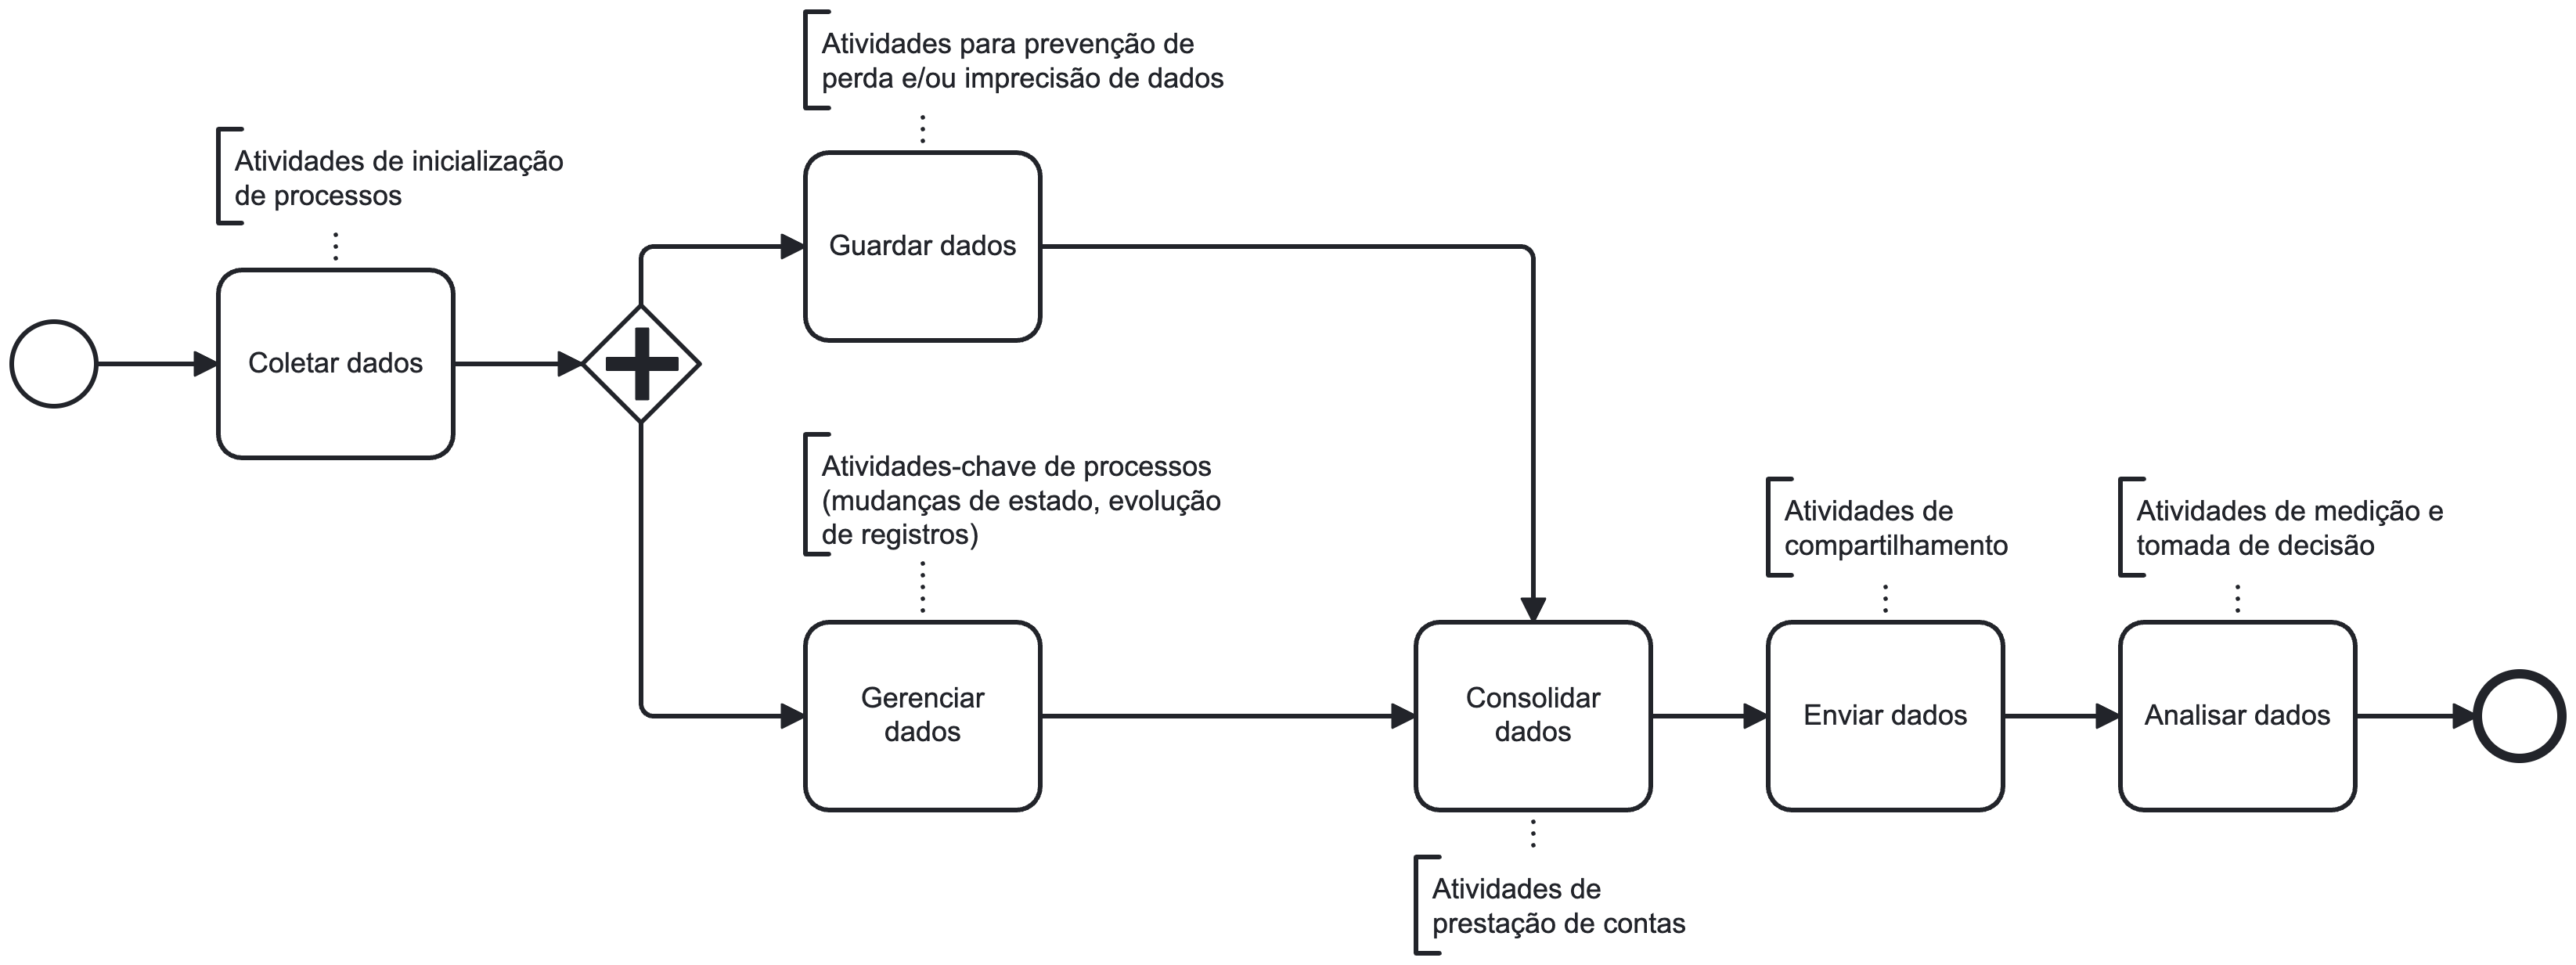
\includegraphics[scale=0.15]{imagens/diagrama_atividades_simplificadas.png}
	\end{center}
	\legend{Fonte: os autores}
\end{figure}

Todos os processos-chave de eixo são iniciados através de uma coleta de dados fundamentais. Em seguida, esses dados são paralelamente guardados de diversas formas e gerenciados — transformados ou manipulados — por atividades-chave. Esses dados, então, são consolidados por coordenadores de eixo para atender demandas de prestação de contas. Eles são enfim compartilhados com a SECTI e analisados conforme o que é preconizado por processos de medição parametrizados pelos objetivos gerais e específicos de cada eixo e por critérios de monitoramento estabelecidos pelo Eixo Transversal. As conclusões dessa atividade de análise de dados apoiam os processos de tomada de decisão do programa.

Constatamos, ainda, que as atividades-chave supracitadas podem ser classificadas como parte de conjuntos de atividades de dois distintos domínios de problemas:

\begin{enumerate}
  \item Problemas da Ponta Inicial;
  \item Problemas da Ponta Final.
\end{enumerate}

\begin{figure}[h]
	\caption{\label{rep_dominios}Domínios de cada conjunto de atividades}
	\begin{center}

  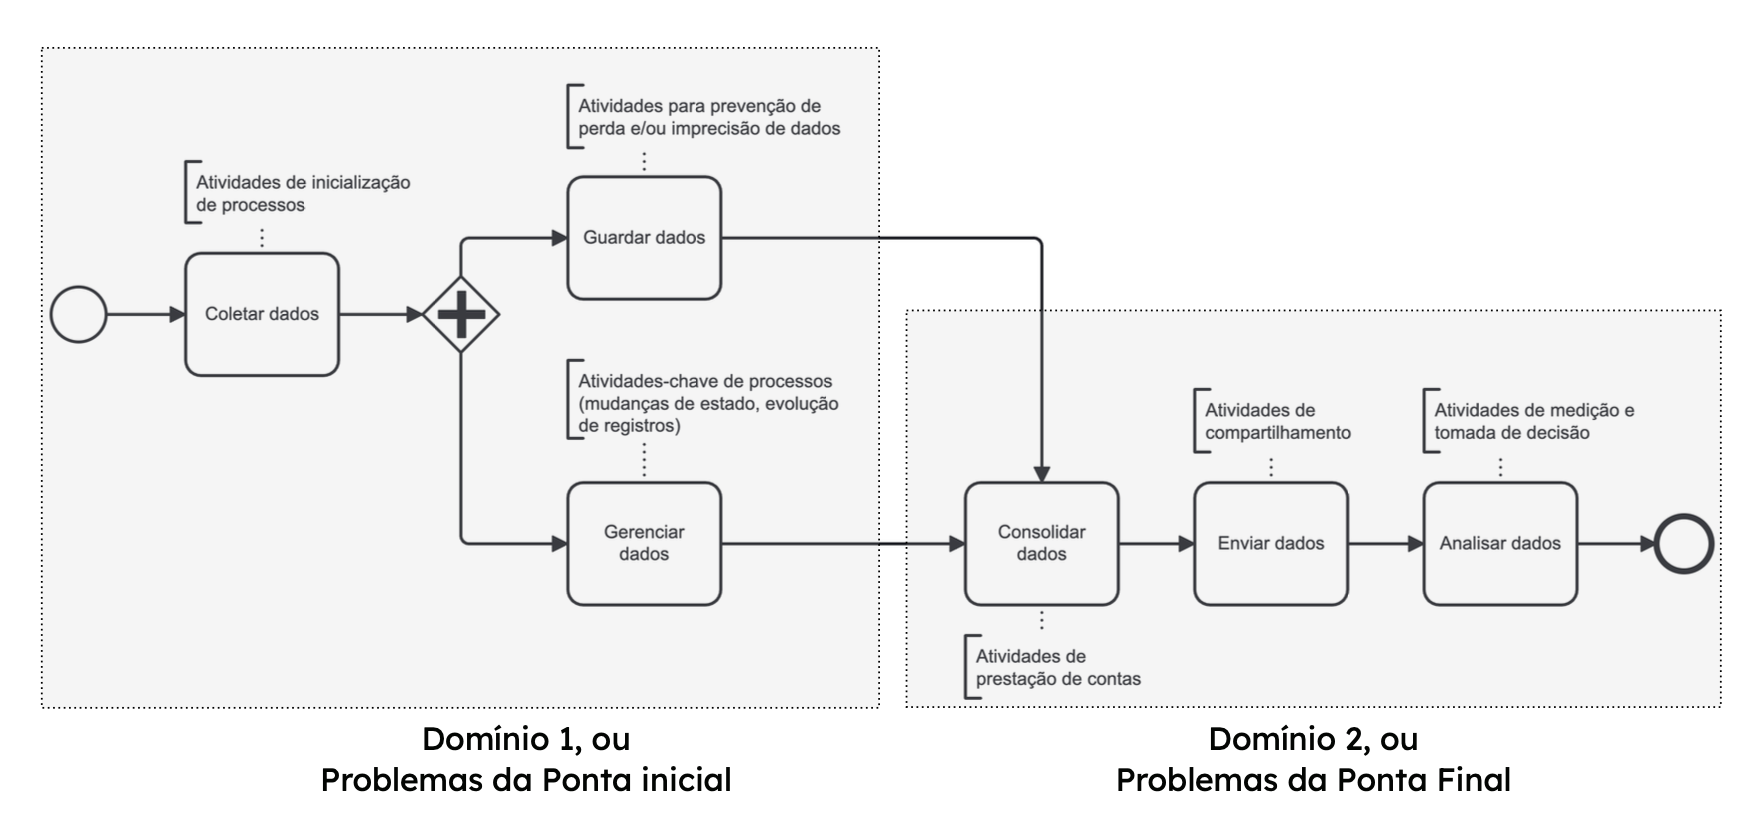
\includegraphics[scale=0.5]{imagens/diagrama_dominios_problemas.png}
	\end{center}
	\legend{Fonte: os autores}
\end{figure}


O Domínio 1, também denominado como Problemas da Ponta Inicial, engloba os problemas de sistemas de informação durante a execução de atividades de operacionalização do programa Sukatech. Neste domínio, identificamos dois grandes problemas:

\begin{itemize}
  \item \textbf{Problema 1.1:} Indisponibilidade de módulos no sistema de software utilizado pela Programando o Futuro para administração de CRCs que contemplem requisitos específicos de todos os eixos do programa Sukatech;
  \item \textbf{Problema 1.2:} Dependência de sistemas manuais de organização de arquivos e pastas para o gerenciamento de dados de eixo (e.g. uso extensivo de Google Drive para administrar documentos de desfazimento no Eixo 1 - Cadeia Produtiva, de registros de turma no Eixo 2 - Capacitação e Empreendedorismo, de campanhas do Eixo 3 - Educação Ambiental).
\end{itemize}

Constatamos, ainda, que esses dois problemas estão interconectados: o Problema 1.1 provoca o Problema 1.2. Notamos, ainda, que as operações dos três eixos do programa Sukatech têm graus de manualidade (isto é, o quão manual é coleta, guarda e gerência de dados) variados: o Eixo 1 - Cadeia Produtiva é o eixo com maior grau de informacionalização uma vez que a Programando o Futuro o executa a partir de um sistema de software próprio responsável por coletar, guardar e gerenciar informações sobre doações, desfazimentos, desmanufaturas e reciclagem de todos os CRCs que a organização opera. O Eixo 2 - Capacitação e Empreendedorismo é gerenciado primariamente a partir de diversas pastas e documentos hospedados no Google Drive. O Eixo 3 - Educação Ambiental também opera em um alto nível de manualidade, mas algumas de suas atividades (e.g. coletas de campanhas) são cobertos pelos sistemas formalizados e amplamente utilizados por atividades do Eixo 1.

O Domínio 2, também denominado como Problemas da Ponta Final, abrange os problemas de sistemas de informação de atividades de gerenciamento e planejamento estratégico do programa Sukatech. Elencamos seis principais problemas:

\begin{itemize}
  \item \textbf{Problema 2.1:} Uso extensivo de planilhas criadas, consolidadas e administradas manualmente para processos de prestação de contas;
  \item \textbf{Problema 2.2:} Trânsito lento de dados entre sistemas administrados pela Programando o Futuro e portais de informação compartilhados com a SECTI;
  \item \textbf{Problema 2.3:} Manipulação acidental de dados inconsistentes e/ou disformes;
  \item \textbf{Problema 2.4:} Processos complexos, trabalhos e extremamente manuais de transformação dos dados semi estruturados recebidos em:
  \begin{itemize}
    \item Métricas para monitoramento, medição de sucesso e fracasso;
    \item Relatórios-padrão para prestação de contas;
    \item Relatórios personalizados para prestação de contas.
  \end{itemize}
  \item \textbf{Problema 2.5:} Insuficiência de dados para medições-chave;
  \item \textbf{Problema 2.6:} Diagnósticos tardios de problemas operacionais.
\end{itemize}

\begin{figure}[ht]
	\caption{\label{rep_dependencia_dominio_2}Dependências entre problemas do Domínio 2}
	\begin{center}

  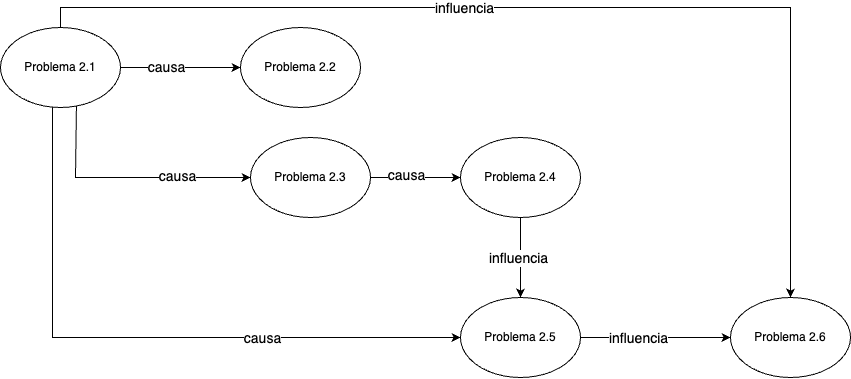
\includegraphics[scale=0.5]{imagens/diagrama_dependencia_dominio_2.png}
	\end{center}
	\legend{Fonte: os autores}
\end{figure}

Constatamos que os seis problemas listados também são inter-relacionados: o Problema 2.1 (consolidação manual de dados) é um fator gerador direto dos problemas 2.2 (trânsito lento de dados), 2.3 (dados inconsistentes e/ou disformes), e 2.5 (dados insuficientes). O Problema 2.3 causa o Problema 2.4 (dificuldades na transformação de dados), que influencia o Problema 2.5. O Problema 2.5, por sua vez, influencia o Problema 2.6 (dignósticos tardios).

Destacamos, ainda, que os diversos relatos de grandes desafios na consolidação de dados do programa Sukatech apontam para uma forte interconexão entre os dois domínios: a ``dívida técnica'' criada pelos problemas do Domínio 1 causa os problemas do Domínio 2. Os problemas do Domínio 2, por conseguinte, perpetuam os problemas do Domínio 1.

\begin{figure}[h]
	\caption{\label{rep_dependencia_dominio}Dependências entre domínios de problemas}
	\begin{center}

  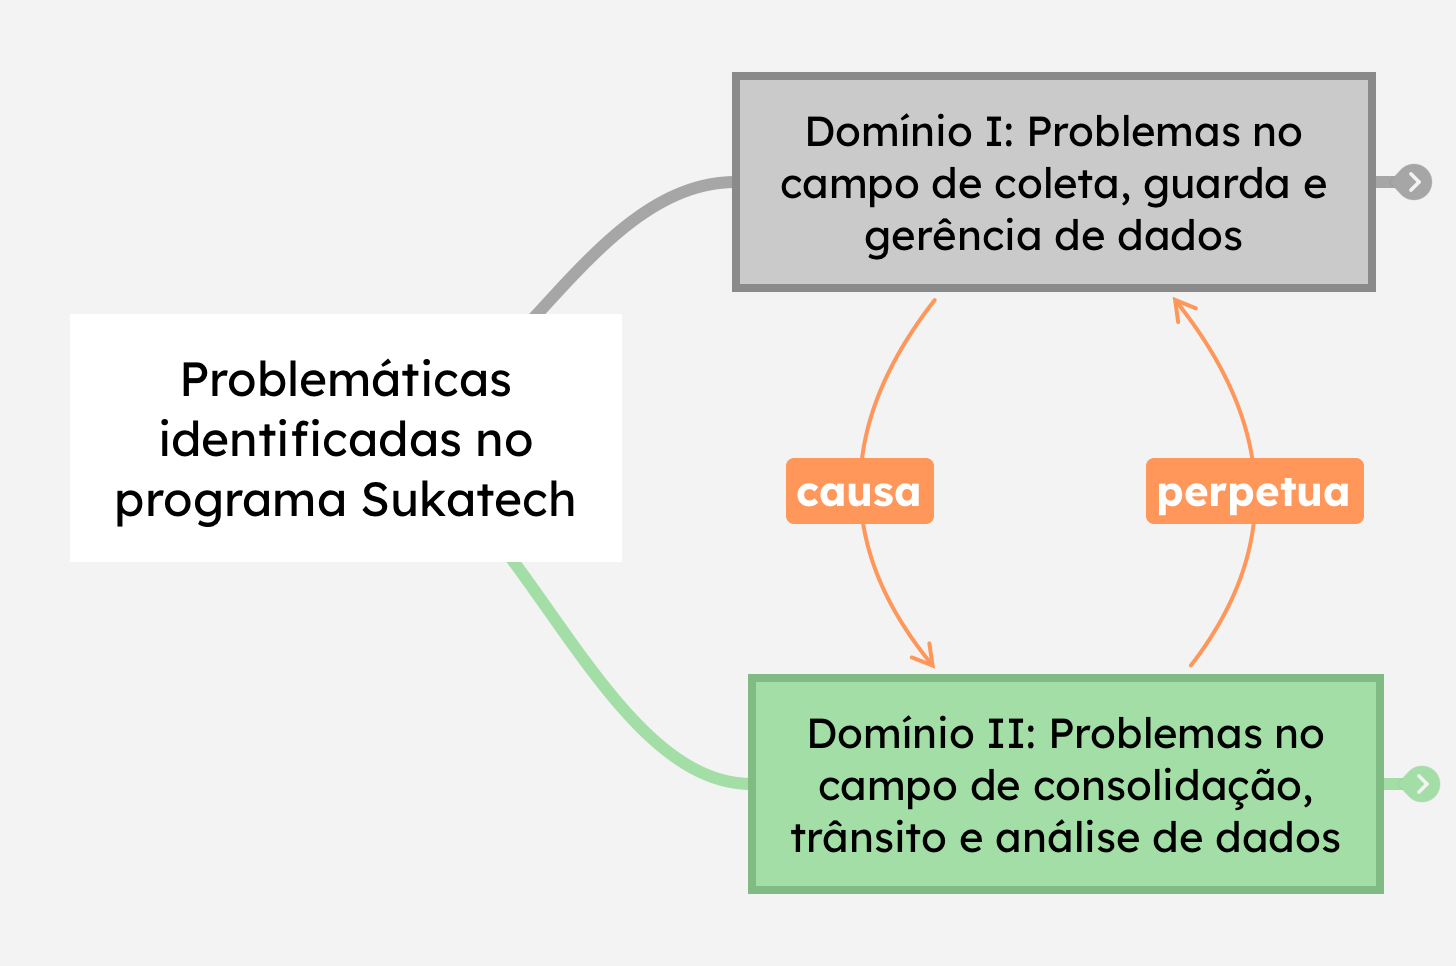
\includegraphics[scale=0.5]{imagens/diagrama_dependencia_dominios.png}
	\end{center}
	\legend{Fonte: os autores}
\end{figure}

\chapter{Mudanças desejadas}

Ressaltamos que, apesar dos problemas citados serem objeto dos objetivos específicos elencados através do Eixo Transversal, observamos uma conexão entre os níveis mais estratégicos da gestão do Sukatech e os níveis operacionais.

Ao realizar o mapeamento de metas, indicadores e fontes apontadas no Plano de Trabalho do programa Sukatech e observar ciclos mensais de prestação de contas, notamos que indicadores qualitativos (e.g. reforma realizada) e indicadores quantitativos (e.g. número de estudantes certificados) não são explicitamente acompanhados por parâmetros bem definidos de progresso, regresso, sucesso ou fracasso. Também destacamos a ausência da formalização de um processo que alinhe, entre níveis gerenciais e operacionais, expectativas e prioridades.

Acreditamos que a falta de estrutura nos processos de medição do programa Sukatech comprometa significativamente os processos de tomada de decisão.

Visando apoiar o crescimento e o amadurecimento do programa, 

\chapter{Mudanças consideradas, mas não incluídas}
\section{Domínio 1 - Problemas da Ponta Inicial}
\begin{itemize}
  \item Documentação de todos os processos operacionais e gerenciais do programa Sukatech, registrando a forma atual de tais processos (\textit{as is}) juntamente ao seu estado desejado (\textit{to be}), classificando-os de acordo a sua maturidade de implementação através da análise da distância entre estado (\textit{as is}) e estado (\textit{to be});
  \item Especificação e desenvolvimento de módulos abrigando requisitos e necessidades para rastreamento das atividades do Eixos 2 e 3 para o sistema utilizado pela Programando o Futuro;
  \item Automatização do processo de criação de planilhas de eixo através do uso de scripts conectados às APIs dos sistemas utilizados pela Programando o Futuro e/ou soluções de automação robótica de processos (Robotic Process Automation — RPA).
\end{itemize}

\section{Domínio 2 - Problemas da Ponta Final}

\begin{itemize}
  \item Automatização do processo de consolidação de planilhas de eixo em uma planilha única para a prestação de contas mensal com a SECTI através do uso de scripts e/ou soluções de RPA;
  \item Normalização e enriquecimento de dados coletados através do cruzamento desses dados com bancos de dados abertos (por exemplo, Wikidata) através da utilização do software OpenRefine;
  \item Sofisticação da análise de dados do programa Sukatech através da mineração de dados, empregando técnicas de análise de sentimentos e análise de agrupamento de dados.
\end{itemize}


\begin{figure}[h]
	\caption{\label{rep_solucoes}Soluções consideradas}
	\begin{center}

  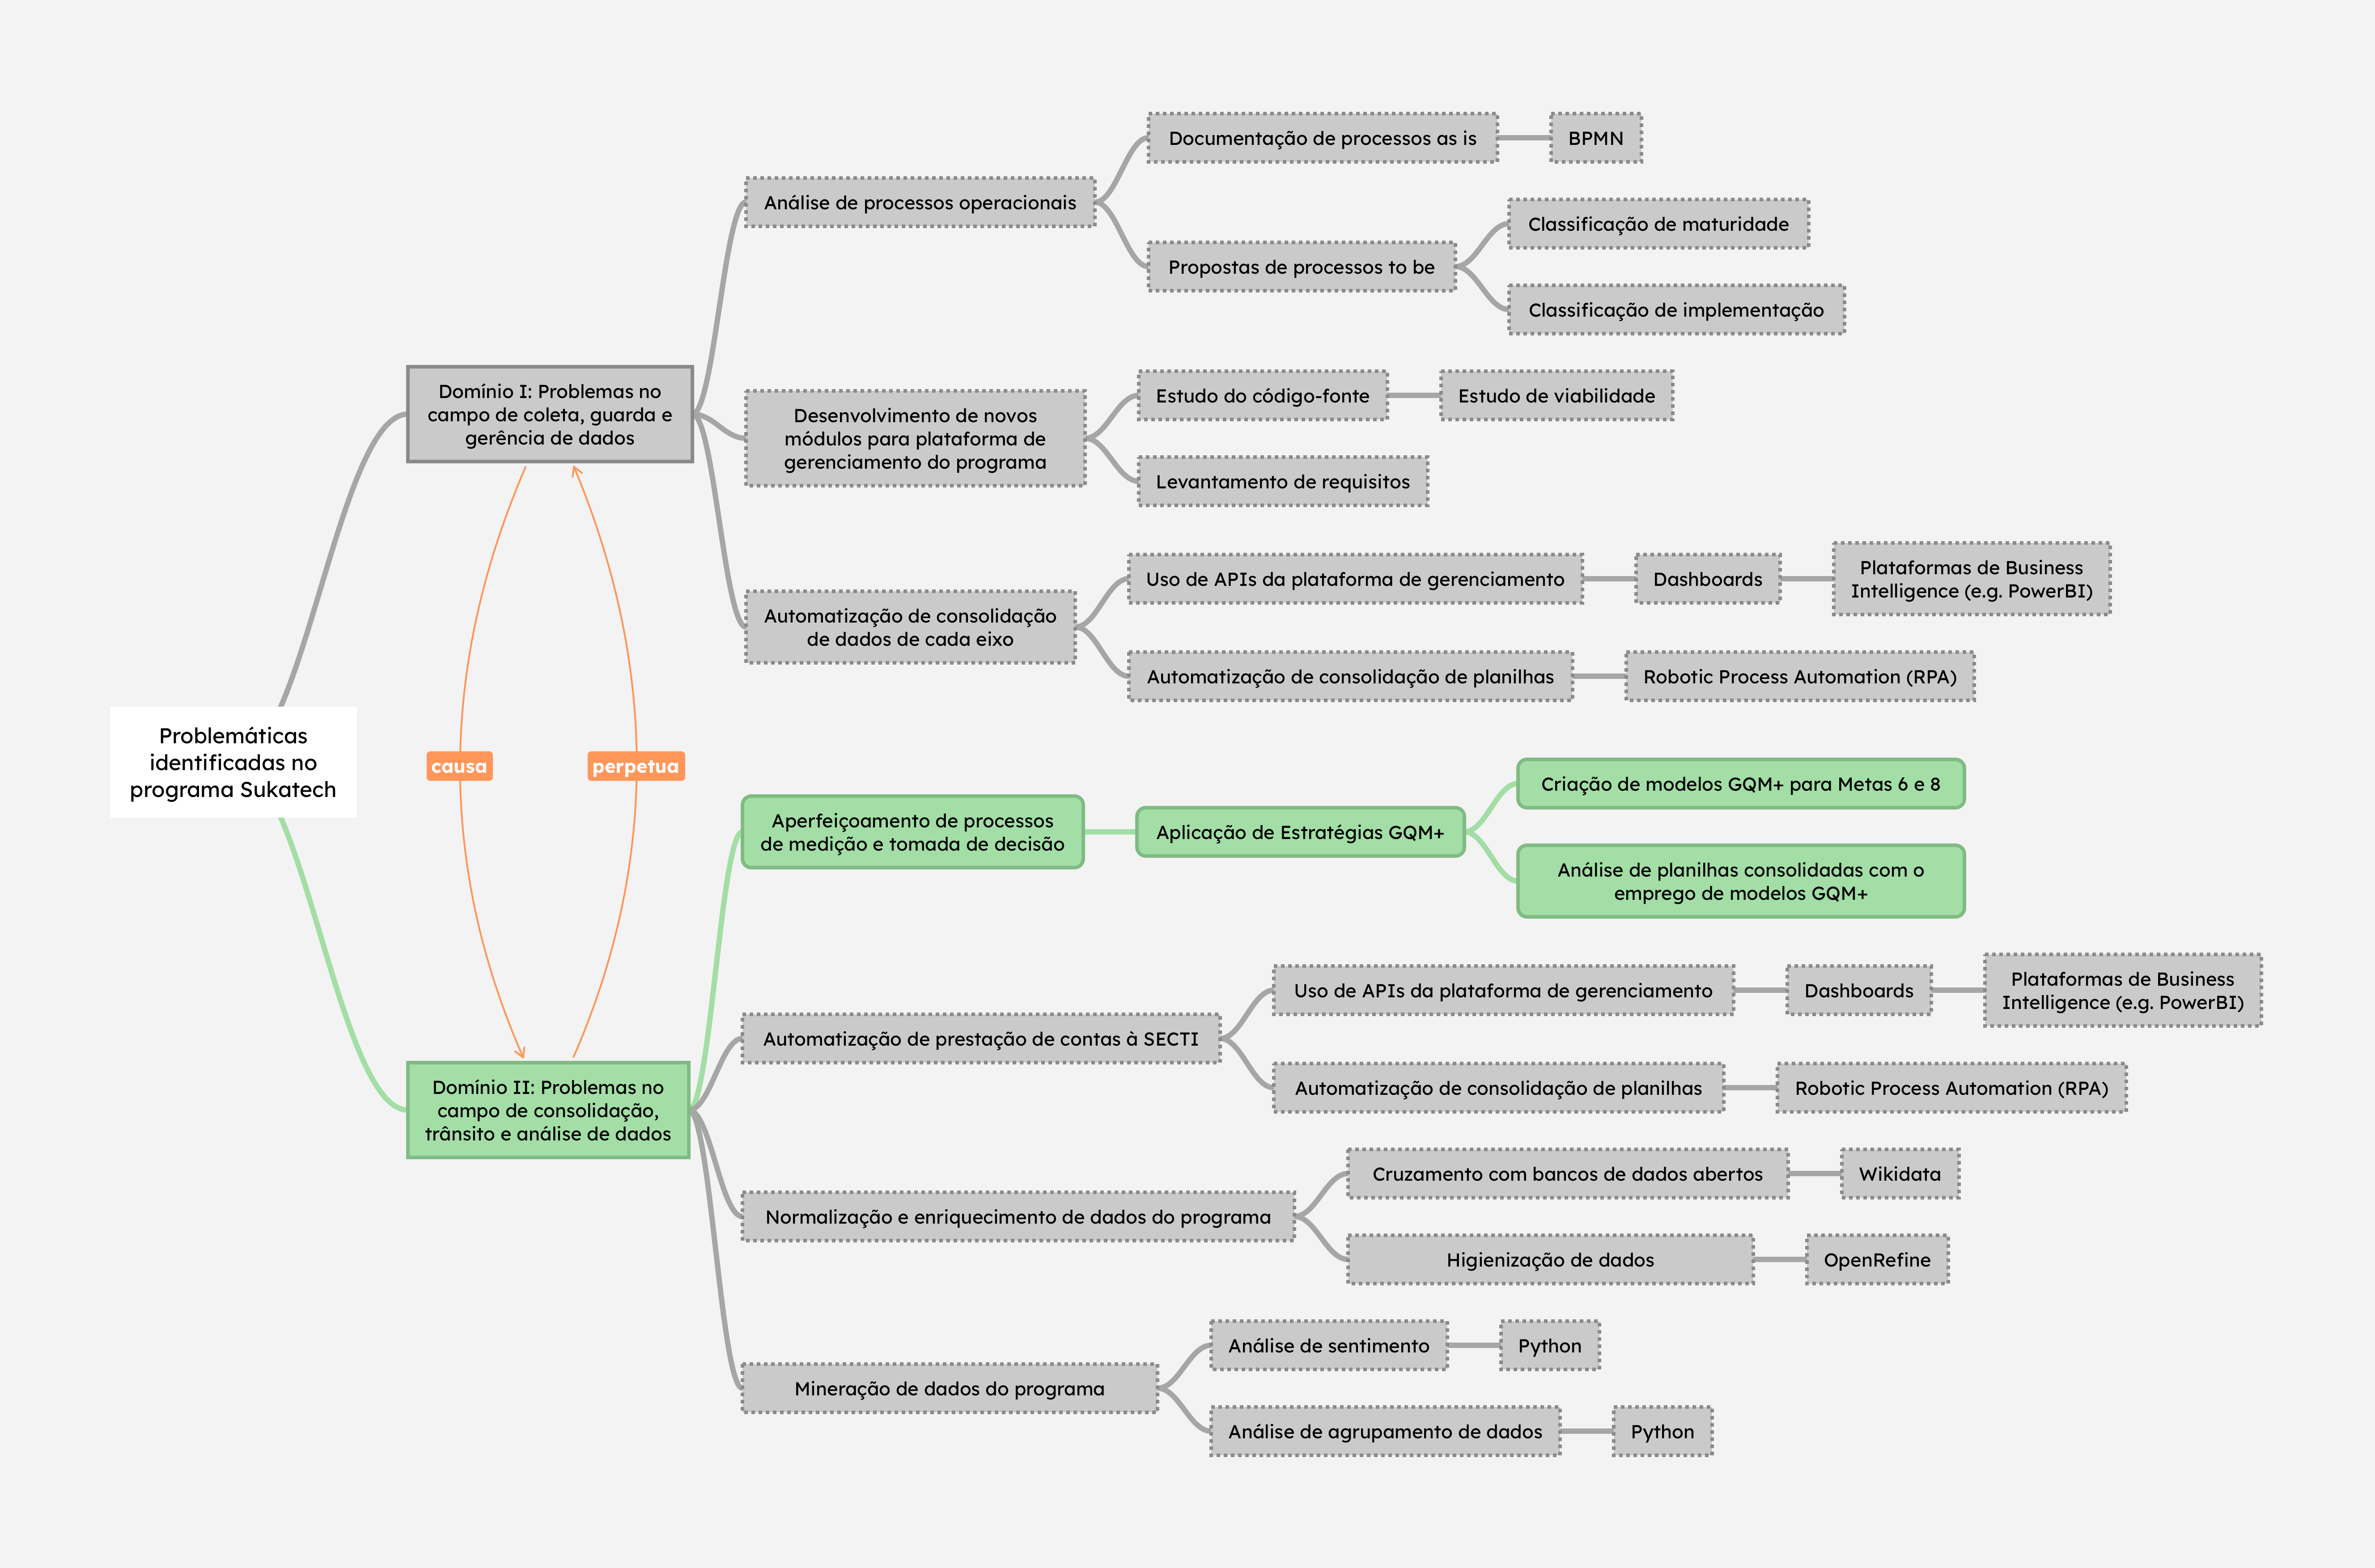
\includegraphics[scale=0.5]{imagens/diagrama_solucoes_consideradas.png}
	\end{center}
	\legend{Fonte: os autores}
\end{figure}

\chapter{Suposições e limitações}



% ----------------------------------------------------------
% Capitulo com exemplos de comandos inseridos de arquivo externo 
% ----------------------------------------------------------

% ----------------------------------------------------------
% Parte de resultados
% ----------------------------------------------------------
\part{Sistema \textit{to be}}
\chapter{Estratégias GQM+}
\chapter{Cenários de aplicação}
\chapter{Análise de impacto}
\section{Impactos operacionais}
\section{Impactos organizacionais}
\section{Impactos durante o desenvolvimento}
\chapter{Análise do sistema proposto}
\section{Benefícios}
\section{Desvantagens e limitações}



% ---
% Finaliza a parte no bookmark do PDF
% para que se inicie o bookmark na raiz
% e adiciona espaço de parte no Sumário
% ---
\phantompart

% ---
% Conclusão
% ---
\chapter{Conclusão}
% ---

\lipsum[31-33]

% ----------------------------------------------------------
% ELEMENTOS PÓS-TEXTUAIS
% ----------------------------------------------------------
\postextual

% ----------------------------------------------------------
% Referências bibliográficas
% ----------------------------------------------------------
\bibliography{abntex2-modelo-references}

% ----------------------------------------------------------
% Glossário
% ----------------------------------------------------------
%
% Consulte o manual da classe abntex2 para orientações sobre o glossário.
%
%\glossary

% ----------------------------------------------------------
% Apêndices
% ----------------------------------------------------------

% ---
% Inicia os apêndices
% ---
\begin{apendicesenv}

% Imprime uma página indicando o início dos apêndices
\partapendices

% ----------------------------------------------------------
\chapter{Quisque libero justo}
% ----------------------------------------------------------

\lipsum[50]

% ----------------------------------------------------------
\chapter{Nullam elementum urna vel imperdiet sodales elit ipsum pharetra ligula
ac pretium ante justo a nulla curabitur tristique arcu eu metus}
% ----------------------------------------------------------
\lipsum[55-57]

\end{apendicesenv}
% ---


% ----------------------------------------------------------
% Anexos
% ----------------------------------------------------------

% ---
% Inicia os anexos
% ---
\begin{anexosenv}

% Imprime uma página indicando o início dos anexos
\partanexos

% ---
\chapter{Morbi ultrices rutrum lorem.}
% ---
\lipsum[30]

% ---
\chapter{Cras non urna sed feugiat cum sociis natoque penatibus et magnis dis
parturient montes nascetur ridiculus mus}
% ---

\lipsum[31]

% ---
\chapter{Fusce facilisis lacinia dui}
% ---

\lipsum[32]

\end{anexosenv}

%---------------------------------------------------------------------
% INDICE REMISSIVO
%---------------------------------------------------------------------

\phantompart

\printindex

%---------------------------------------------------------------------
% Formulário de Identificação (opcional)
%---------------------------------------------------------------------
\chapter*[Formulário de Identificação]{Formulário de Identificação}
\addcontentsline{toc}{chapter}{Exemplo de Formulário de Identificação}
\label{formulado-identificacao}

Exemplo de Formulário de Identificação, compatível com o Anexo A (informativo)
da ABNT NBR 10719:2015. Este formulário não é um anexo. Conforme definido na
norma, ele é o último elemento pós-textual e opcional do relatório.

\bigskip

\begin{tabular}{|p{9cm}|p{5cm}|}
\hline
\multicolumn{2}{|c|}{\textbf{\large Dados do Relatório Técnico e/ou científico}}\\
\hline
\multirow{4}{10cm}[24pt]{Título e subtítulo}& Classificação de segurança\\
                   & \\
                   \cline{2-2}
                   & No.\\
                   & \\
				
\hline
Tipo de relatório & Data\\
\hline
Título do projeto/programa/plano & No.\\
\hline
\multicolumn{2}{|l|}{Autor(es)} \\
\hline
\multicolumn{2}{|l|}{Instituição executora e endereço completo} \\
\hline
\multicolumn{2}{|l|}{Instituição patrocinadora e endereço completo} \\
\hline
\multicolumn{2}{|l|}{Resumo}\\[3cm]
\hline
\multicolumn{2}{|l|}{Palavras-chave/descritores}\\
\hline
\multicolumn{2}{|l|}{
Edição \hfill No. de páginas \hfill No. do volume \hfill Nº de classificação \phantom{XXXX}} \\
\hline
\multicolumn{2}{|l|}{
ISSN \hfill \hfill Tiragem \hfill Preço \phantom{XXXXXXXX}} \\
\hline
\multicolumn{2}{|l|}{Distribuidor} \\
\hline
\multicolumn{2}{|l|}{Observações/notas}\\[3cm]
\hline
\end{tabular}

\end{document}

